\PassOptionsToPackage{unicode=true}{hyperref} % options for packages loaded elsewhere
\PassOptionsToPackage{hyphens}{url}
%
\documentclass[english,doc]{apa6}
\usepackage{lmodern}
\usepackage{amssymb,amsmath}
\usepackage{ifxetex,ifluatex}
\usepackage{fixltx2e} % provides \textsubscript
\ifnum 0\ifxetex 1\fi\ifluatex 1\fi=0 % if pdftex
  \usepackage[T1]{fontenc}
  \usepackage[utf8]{inputenc}
  \usepackage{textcomp} % provides euro and other symbols
\else % if luatex or xelatex
  \usepackage{unicode-math}
  \defaultfontfeatures{Ligatures=TeX,Scale=MatchLowercase}
\fi
% use upquote if available, for straight quotes in verbatim environments
\IfFileExists{upquote.sty}{\usepackage{upquote}}{}
% use microtype if available
\IfFileExists{microtype.sty}{%
\usepackage[]{microtype}
\UseMicrotypeSet[protrusion]{basicmath} % disable protrusion for tt fonts
}{}
\IfFileExists{parskip.sty}{%
\usepackage{parskip}
}{% else
\setlength{\parindent}{0pt}
\setlength{\parskip}{6pt plus 2pt minus 1pt}
}
\usepackage{hyperref}
\hypersetup{
            pdftitle={If mathematical psychology did not exist we would need to invent it: A case study in cumulative theoretical development in psychology},
            pdfkeywords={X},
            pdfborder={0 0 0},
            breaklinks=true}
\urlstyle{same}  % don't use monospace font for urls
\usepackage{graphicx,grffile}
\makeatletter
\def\maxwidth{\ifdim\Gin@nat@width>\linewidth\linewidth\else\Gin@nat@width\fi}
\def\maxheight{\ifdim\Gin@nat@height>\textheight\textheight\else\Gin@nat@height\fi}
\makeatother
% Scale images if necessary, so that they will not overflow the page
% margins by default, and it is still possible to overwrite the defaults
% using explicit options in \includegraphics[width, height, ...]{}
\setkeys{Gin}{width=\maxwidth,height=\maxheight,keepaspectratio}
\setlength{\emergencystretch}{3em}  % prevent overfull lines
\providecommand{\tightlist}{%
  \setlength{\itemsep}{0pt}\setlength{\parskip}{0pt}}
\setcounter{secnumdepth}{0}

% set default figure placement to htbp
\makeatletter
\def\fps@figure{htbp}
\makeatother

% Manuscript styling
\usepackage{upgreek}
\captionsetup{font=singlespacing,justification=justified}

% Table formatting
\usepackage{longtable}
\usepackage{lscape}
% \usepackage[counterclockwise]{rotating}   % Landscape page setup for large tables
\usepackage{multirow}		% Table styling
\usepackage{tabularx}		% Control Column width
\usepackage[flushleft]{threeparttable}	% Allows for three part tables with a specified notes section
\usepackage{threeparttablex}            % Lets threeparttable work with longtable

% Create new environments so endfloat can handle them
% \newenvironment{ltable}
%   {\begin{landscape}\begin{center}\begin{threeparttable}}
%   {\end{threeparttable}\end{center}\end{landscape}}
\newenvironment{lltable}{\begin{landscape}\begin{center}\begin{ThreePartTable}}{\end{ThreePartTable}\end{center}\end{landscape}}

% Enables adjusting longtable caption width to table width
% Solution found at http://golatex.de/longtable-mit-caption-so-breit-wie-die-tabelle-t15767.html
\makeatletter
\newcommand\LastLTentrywidth{1em}
\newlength\longtablewidth
\setlength{\longtablewidth}{1in}
\newcommand{\getlongtablewidth}{\begingroup \ifcsname LT@\roman{LT@tables}\endcsname \global\longtablewidth=0pt \renewcommand{\LT@entry}[2]{\global\advance\longtablewidth by ##2\relax\gdef\LastLTentrywidth{##2}}\@nameuse{LT@\roman{LT@tables}} \fi \endgroup}

% \setlength{\parindent}{0.5in}
% \setlength{\parskip}{0pt plus 0pt minus 0pt}

% \usepackage{etoolbox}
\makeatletter
\patchcmd{\HyOrg@maketitle}
  {\section{\normalfont\normalsize\abstractname}}
  {\section*{\normalfont\normalsize\abstractname}}
  {}{\typeout{Failed to patch abstract.}}
\makeatother
\shorttitle{Psychological theory}
\author{Danielle J. Navarro\textsuperscript{1}}
\affiliation{
\vspace{0.5cm}
\textsuperscript{1} School of Psychology, University of New South Wales}
\authornote{This manuscript is based on conversations with Berna Dezever and many others. I want to specifically note Berna's contribution in this initial submission as she will likely be a coauthor on any published version. At the current point in development she has not had the opportunity to provide input and (as a way of assuming sole responsibilities for any errors in the current version) I have not listed her as a coauthor at this stage.


Correspondence concerning this article should be addressed to Danielle J. Navarro, School of Psychology, University of New South Wales, Kensington 2052, Sydney, Australia. E-mail: d.navarro@unsw.edu.au}
\keywords{X\newline\indent Word count: X}
\usepackage{csquotes}
\usepackage{amsmath}
\ifnum 0\ifxetex 1\fi\ifluatex 1\fi=0 % if pdftex
  \usepackage[shorthands=off,main=english]{babel}
\else
  % load polyglossia as late as possible as it *could* call bidi if RTL lang (e.g. Hebrew or Arabic)
  \usepackage{polyglossia}
  \setmainlanguage[]{english}
\fi

\title{If mathematical psychology did not exist we would need to invent it: A case study in cumulative theoretical development in psychology}

\date{}

\abstract{
Lorem ipsum dolor sit amet, consectetur adipiscing elit, sed do eiusmod tempor incididunt ut labore et dolore magna aliqua. Sollicitudin nibh sit amet commodo. Malesuada pellentesque elit eget gravida cum. Magna fermentum iaculis eu non. Tempus imperdiet nulla malesuada pellentesque elit eget gravida. Donec massa sapien faucibus et molestie ac. Non blandit massa enim nec dui. Tellus in hac habitasse platea dictumst vestibulum rhoncus. Massa sed elementum tempus egestas sed sed. Pretium fusce id velit ut tortor pretium viverra suspendisse. At quis risus sed vulputate. Eget sit amet tellus cras adipiscing enim. Amet risus nullam eget felis. Lectus urna duis convallis convallis tellus id.
}

\begin{document}
\maketitle

\newpage

\begin{quote}
\emph{Those outside the field, on hearing the term mathematical psychology, often react with the raised eyebrows reserved for oxymora} (Shepard, 2004, p. 1)
\end{quote}

\vspace*{12pt}

\hypertarget{introduction}{%
\section{Introduction}\label{introduction}}

In 1987 Roger Shepard published a short paper in \emph{Science} with the ambitious title \enquote{Toward a Universal Law of Generalization for Psychological Science} (Shepard, 1987). Drawing on extensive work in the empirical literature on stimulus generalization across many species, he asserted the claim that the form of any stimulus generalization function shouold be approximately exponential in form, when measured with respect to an appropriately formulated stimulus representation. His paper begins with the following remark (p.~1317):

\begin{quote}
The tercentenary of the publication, in 1687, of Newton's \emph{Principia} prompts the question of whether psychological science has any hope of achieving a law that is comparable in generality (if not in predictive accuracy) to Newton's universal law of gravitation. Exploring the direction that currently seems most favorable for an affirmative answer, I outline empirical evidence an a theoretical rationale in support of a tentative candidate for a universal law of generalization
\end{quote}

\noindent
Shepard's claim in the original paper was remarkable in scope. He drew on data from several terrestrial species (e.g., humans, pigeons, rats) and across many stimulus domains (e.g., visual, auditory), data that had hitherto been considered unrelated. To spot the connection between these data, Shepard used statistical insights from the similarity modelling literature. He noted that the apparent noninvariance of observed stimulus generalisation functions stemmed largely from the fact that response data were previously analysed with respect to the physical dissimilarities of the stimulus. When the same responses were replotted as a function of distance in a psychological space contructed by multidimensional scaling, he found that the form of the stimulus generalisation was remarkably regular in shape, as shown on the left side of Figure 1.



\begin{figure}[t]
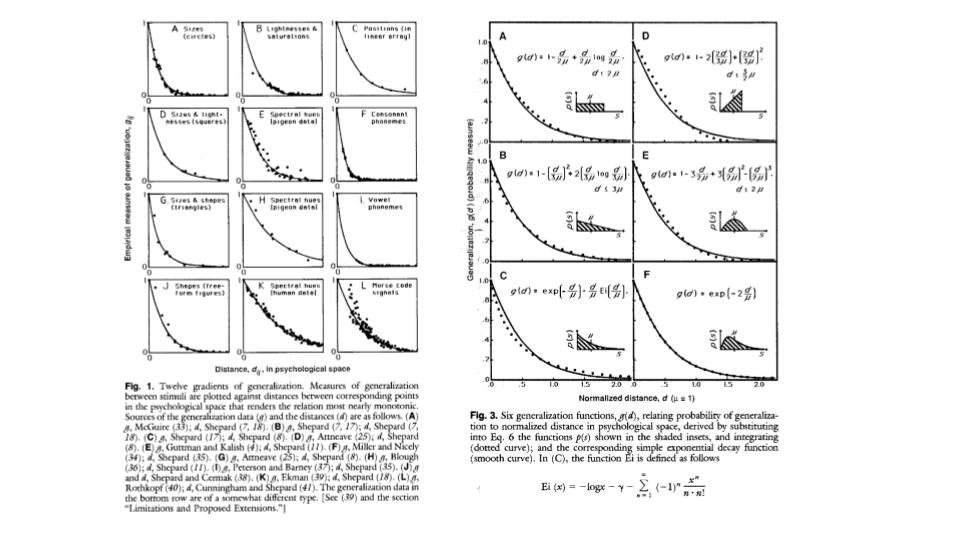
\includegraphics[width=6.4in]{shepard} \caption{Two of the figures from Shepard's (1987) paper on stimulus generalisation. On the left, his Fig 1 shows the empirical evidence for an exponential law and on the right his Fig 3 outlines his theoretical claim. {[}Note: higher resolution versions will be provided in the final version and permission will be obtained to reproduce the originals{]}}\label{fig:unnamed-chunk-1}
\end{figure}

Taken by itself Shepard's empirical discovery would have been impressive. However, not content merely to reanalyse existing the data to discover the underlying invariance and thereby unify several distinct strands of research, Shepard went on to provide a theoretical explanation for \emph{why} we should expect to find this invariance. The theory was surprisingly simple: the learner presumes there exists some unknown \emph{consequential} region of the stimulus space across which roughly the same properties hold (e.g., things that look like apples will probably taste the same as one another). Encountering a single stimulus that entails a particular consequence, the learner's task is to infer the location, shape and size of the consequential region itself. Naturally this is an underconstrained problem, as there are an infinite number of possible regions that might correspond to the true consequential region. Nevertheless, Shepard showed that under a quite range of assumptions that the learner might make about the nature of consequential regions, the shape of the \emph{generalization} function across the stimulus space ends up approximately exponential, shown on the right side of Figure 1.

Since its publication in 1987, Shepard's paper has been cited approximately 2500 times according to Google Scholar, no small feat for a theoretical paper that presented no new empirical data and whose content is almost entirely devoted to the derivation of a formal relation between one unobservable quantity (distance between two items psychological space) and another (the probability two items fall in the same region). The universal law featured prominently in a special issue of Brain and Behavior Sciences in 2001, as well as a first person retrospective written 17 years later (Shepard, 2004). It is rightly considered one of the most important works in mathematical psychology, and indeed all of coognitive science. In this special issue devoted to the prospects for theoretical development in psychology, I can think of no better case study to motivate our remarks. My goal in this paper is to discuss the role that theory can play in the development of psychological science, using Shepard's law to illustrate.

\hypertarget{what-a-theory-is-not}{%
\section{What a theory is not}\label{what-a-theory-is-not}}

Reading Shepard's original 1987 paper and the 2004 retrospective, some surprising characteristics of his theoretical work stand out. First, the theoretical development was largely post hoc. The paper does not collect new data, and indeed the main empirical results reported in the paper (left hand side of Figure 1) were based on a reanalysis of existing data. Second, the paper reports no hypothesis tests or indeed any statistical inference of any kind. There are no p-values, no Bayes factors, nor any confidence intervals or their Bayesian equivalents. Third, the paper does not outline any specific novel prediction about the result of future experiments. Though the paper makes a strong claim that the exponential law should hold broadly it does prescribe how tests of this prediction should be constructed.

Given the current climate in psychological science, all three of these might seem somewhat surprising, perhaps even a form of ``questionable'' research practice. In the current zeitgeist, statistical tests are considered essential, post hoc theorising is a questionable research practice, and prediction is considered the central goal of theory. Judged by the standards currently used to assess psychological research Shepard's paper fares quite poorly. One might be tempted to ask how Shepard managed to get the paper published at all, much less to have it established as one of the most influential theoretical works in cognitive science! Or alternatively, to take a different perspective, perhaps these standards are ill-suited to the job of assessing theoretical work.

Indeed, one might argue that the success of Shepard's law tells us a great deal about what a theory is not. Novel data, no matter how fascinating or carefully collected, do not make a theoretical contribution. A statistical test, no matter how well constructed, does not encapsulate what a theory does. Perhaps surprisingly, a theory need not make novel predictions. Shepard's theoretical contribution was not the discovery of the exponential law, but rather to explain it. What Shepard's paper did was \emph{systematise} an existing body of empirical findings, separating those aspects to the data that are invariant across studies from that which is not, and provided a precisely stated mathematical formalism that did more than merely summarise the data. Shepard's theory asserts that the form of generalization curves are exponential, but the exponential form is not a theoretical primitive. The theoretical primitives are the assumptions Shepard made about consequential regions, psychological spaces, and the relationship these things have to stimulus generalization. The exponential law is an \emph{entailment} of the theory, not its substance.

Empirical data, statistical inference and novel predictions are all vital to the scientific process -- of that there is little doubt -- but none of them are substitutes for or synonymous with theoretical development. If so, what might a theory be?

\hypertarget{how-to-make-a-psychological-theory}{%
\section{How to make a psychological theory}\label{how-to-make-a-psychological-theory}}

It is not difficult to list some of the desiderata for a scientific theory. A scientific theory should be \emph{independent of its creator}, for instance. It is difficult to make much use of a theory otherwise. In practice this typically means a theory is mathematical or computational in nature. Similarly, psychological theories should of course make some connection with empirical data, giving some account of the \emph{generative mechanism} that gave rise to those data. Theories should be usable, in the sense of providing other scientists \emph{guidance for future research}. Other criteria could also be named, including falsifiability, simplicity, compatibility with existing literature, generalizability, predictive ability and so on. However, while it is easy to list desiderata and even easier to argue over which elements to such lists are the most important, such ``discussions in the abstract'' rarely provide much guidance to the would-be theoretician. From the perspective of the working scientist, it is perhaps more useful to give concrete examples, and to that end I return to an examination of Shepard's (1987) paper.

\hypertarget{a-theory-can-have-scope-outside-the-measurement-instrument}{%
\subsection{A theory can have scope outside the measurement instrument}\label{a-theory-can-have-scope-outside-the-measurement-instrument}}

One of the key insights in Shepard (1987) is the recognition that stimulus generalization functions that appear extremely irregular at first glance are in fact highly regular when stimuli are represented in an appropriate fashion, as depicted in Figure 2. Generalization to tones is irregular when tones are described in terms of their ordering around the chroma circle, but very smooth when described around the circle of fifths. Similarly, stimulus generalization to colours is irregular with respect the physical wavelenghts of light but is smooth with respect to perceptual colours space (e.g., Ekman 1954). In retrospect this seems an obvious point to cognitive scientists who have built from Shepard's work, and moreover in keeping with philosophical work on the representation of similarity (Goodman 1972). However, at the time Shepard developed the theory, he was faced with a substantive problem of how to extract the \emph{appropriate} stimulus representation to apply a theory to. Nonmetric multidimensional scaling (CITE) as a measurement instrument tool served this purpose for Shepard in 1987, and the smooth empirical curves on the left of Figure 1 all use MDS-estimated psychological spaces to supply the relevant measure of distance on the x-axis.



\begin{figure}[t]
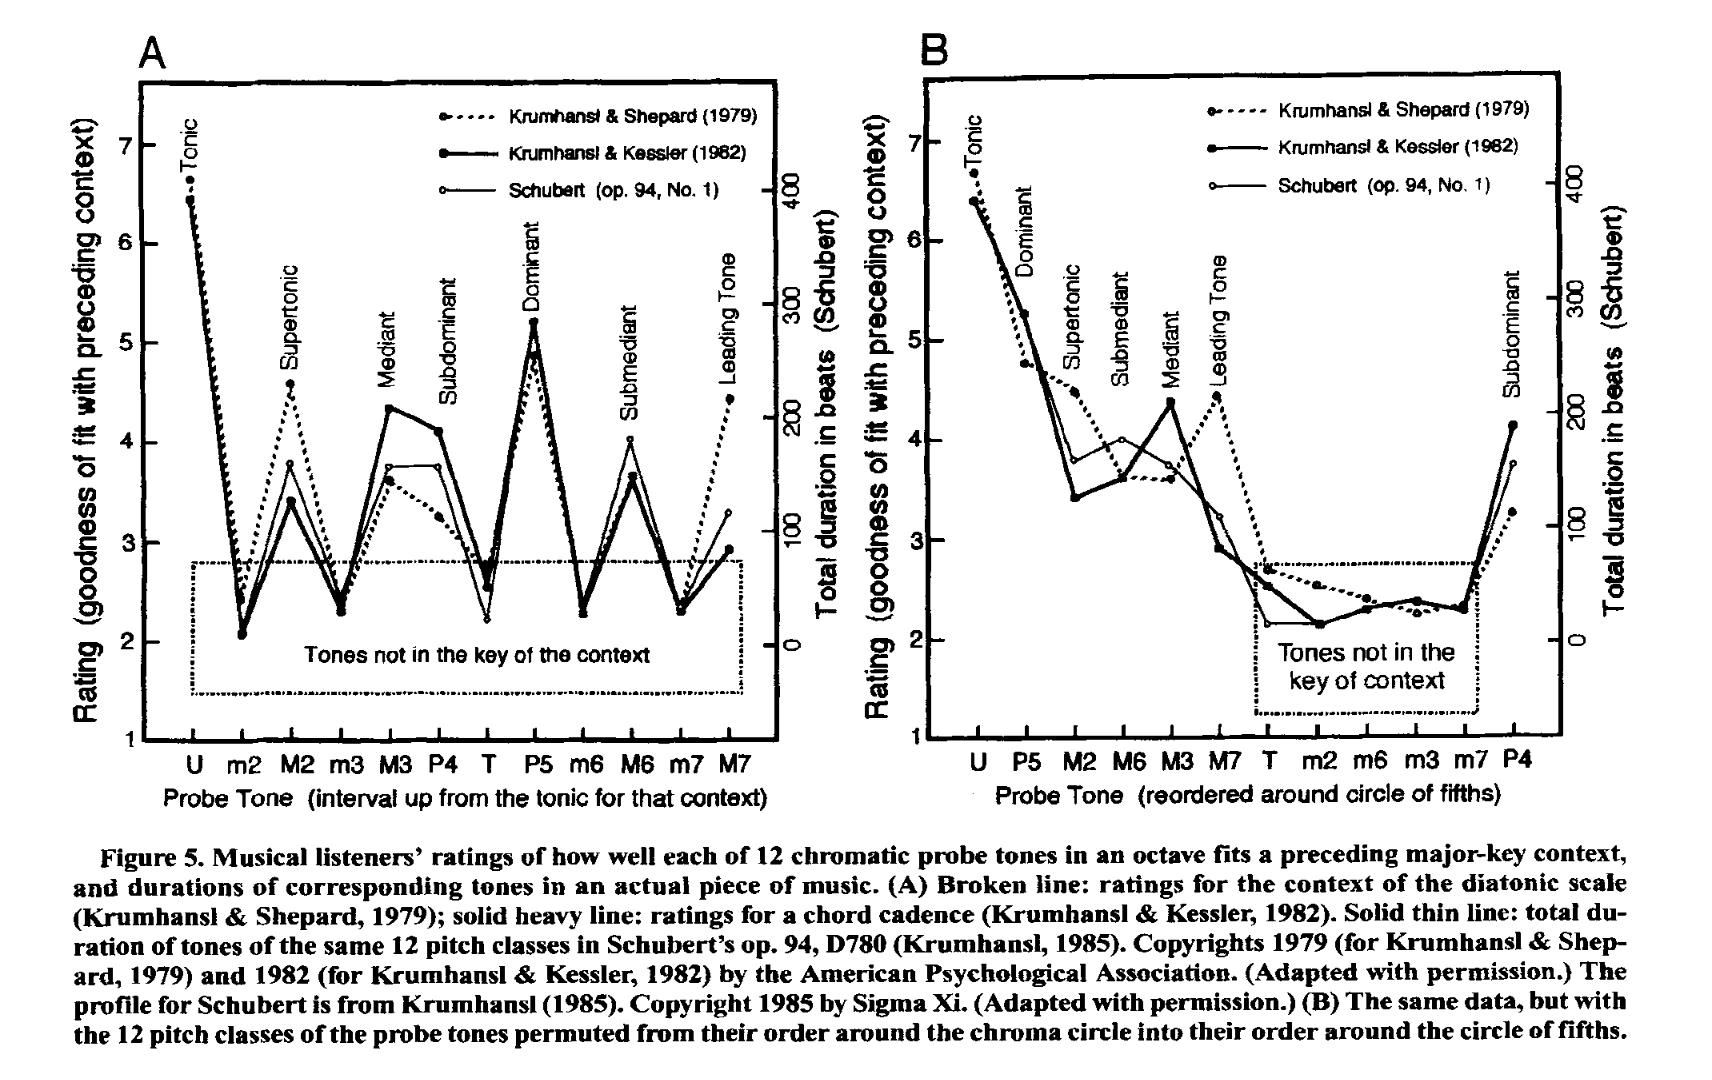
\includegraphics[width=5.71in]{shepard2} \caption{Figure 5 from Shepard's (2004) retrospective account of the universal law, plotting data from previous experiments in the original form (left) and after those same data were recast in terms of constructs relevant to the theory (right). {[}Note: a higher resolution version will be provided in the final version and permission will be obtained to reproduce the originals{]}}\label{fig:unnamed-chunk-2}
\end{figure}

Clearly, without MDS as a measurement tool, Shepard would have found it almost impossible to formulate the empirical regularity with any confidence. However, it is equally clear that MDS is merely a tool used to help define the phenomenon to be explained. It does not define the theory itself, and it quickly became apparent that the scope of Shepard's law applies in situations where MDS does not: shortly after the publication of Shepard's original paper, Russell (1988) demonstrated that the same law holds for stimuli defined in terms of discrete features as well as to the continuous spaces for which Shepard's work was defined, a connection that was later extended by Tenenbaum and Griffiths (2001). While the theoretical framework could not have come into existence without the scaffolding provided by the MDS measurement model, it quickly outgrew any need for this support. Illustrating this, the generalization gradient shown in Figure 3 is neither exponential in superficial form, nor is the underlying stimulus representation a metric space extracted by MDS, yet as Tenenbaum and Griffiths (2001) note, it too can be seen as an entailment of Shepard's theoretical framework.



\begin{figure}[t]
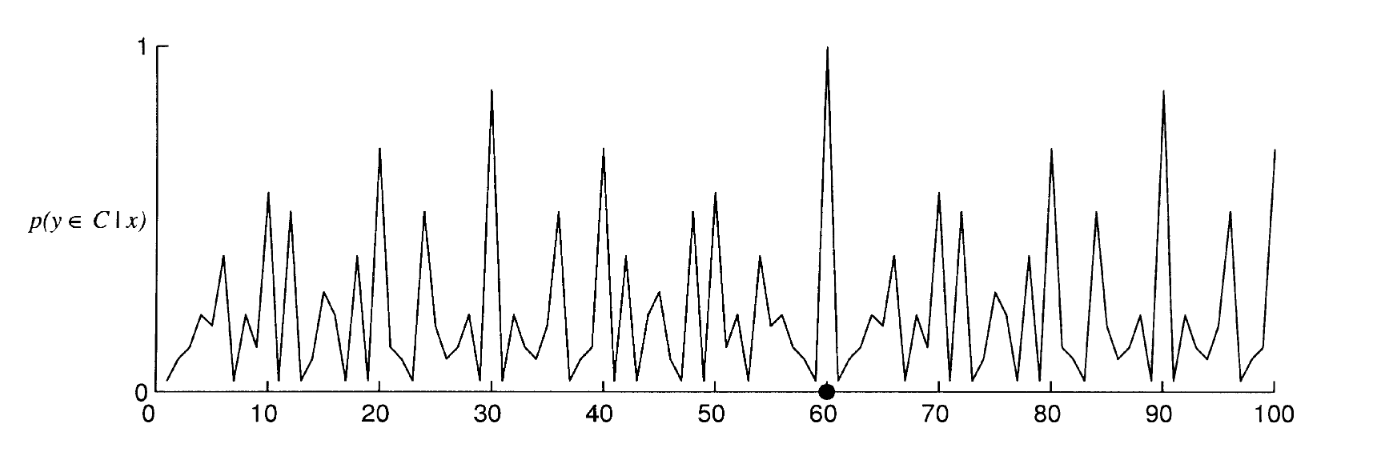
\includegraphics[width=6.07in]{tenenbaum_figure5} \caption{Figure 5 from Tenenbaum and Griffiths' (2001) paper \emph{Generalization, similarity, and Bayesian inference}. {[}Note: a higher resolution version will be provided in the final version and permission will be obtained to reproduce the originals{]}}\label{fig:unnamed-chunk-3}
\end{figure}

\hypertarget{a-theory-should-be-extensible-by-others}{%
\subsection{A theory should be extensible by others}\label{a-theory-should-be-extensible-by-others}}

The original theory of generalization presented by Shepard (1987) was not explicitly framed as Bayesian model of cognition. In his original notation (Equation 2 from the paper) Shepard proposed that the generalization strength for a stimulus located at coordinate \(\mathbf{x} = (x_1, \ldots, x_K)\) in a \(K\)-dimensional space,\footnote{The space is usually endowed with one of the Minkowski distance metrics, most typically the Euclidean distance measure or the city block distance. One of the major contributions Shepard made was to provide a theoretical explanation for why the distance metric varies across stimulus domains, but is a little beyond the scope of the current paper.} when the learner has previously encountered a consequential stimulus located at the origin be expressed as follows:

\begin{equation}
g(\mathbf{x}) = \int_0^\infty p(s) \frac{m(s, \mathbf{x})}{m(s)} ds
\end{equation}

\noindent
where the ratio \(m(s, \mathbf{x})/m(s)\) is a measure describing the probability that a consequential region of size \(s\) contains \(\mathbf{x}\) given that it also contains the consequential stimulus at the origin, and \(p(s)\) is a probability measure that assigns value to regions of size \(s\). Much of Shepard's paper is devoted to solving this integral for various choices of \(p(s)\) and showing that the resulting generalization function \(g(\mathbf{x})\) is approximately exponential in form, and is precisely exponential when \(p(s)\) is the Erlang distribution.

The connection to Bayesian inference was made explicit by Tenenbaum and Griffiths (2001) who recast Shepard's formalism in the following fashion. Where Shepard referred to the notion of a \emph{consequential region} located within a psychological space (with all the geometric connotations that entails), Tenenbaum and Griffiths relaxed this to be a more general \emph{consequential set}. Any specific candidate for the true consequential set was labelled a \emph{hypothesis} \(h\), presumed to belong to a broader \emph{hypothesis space} \(\mathcal{H}\). In their notation, the measure on regions sizes \(p(s)\) was replaced by a Bayesian prior \(p(h)\) defined over the hypothesis space, and Shepard's ratio \(m(s, \mathbf{x})/m(s)\) recast in probabilistic terms also. In their notation, the probability of generalising to a novel stimulus \(y\) given that a consequential stimulus \(x\) has already been observed is formulated as the following Bayesian marginal probability:

\begin{equation}
p(y \in C | x) = \sum_{h : y \in C} p(h|x)
\end{equation}
\noindent
where \(p(h|x)\) is the posterior probability a Bayesian learner assigns to hypothesis \(h\) in light of observing the consequential stimulus \(x\),
\begin{equation}
p(h|x) = \frac{p(x|h)p(h)}{\sum_{h^\prime \in \mathcal{H}} p(x | h^\prime) p(h^\prime)}
\end{equation}

The Bayesian reformulation of Shepard's theory presented by Tenenbaum and Griffiths was more than a superficial change: it allowed them to show how Shepard's theory could itself be generalized in three distinct ways. First, as mentioned earlier, they showed (much like Russell 1988) that Shepard's theory could encompass stimuli that were not representable as points in a metric space: in their notation, this is as accomplished by substituting a new hypothesis space \(\mathcal{H}\). Second, this formulation allowed the theory to naturally accommodate inductive generalization problems in which the learner has encountered more than one consequential stimulus. If a set of \(n\) stimuli \(\mathbf{x} = (x_1, \ldots, x_n)\) are generated in a (conditionally) independent fashion, the likelihood \(p(\mathbf{x}|h)\) factorises and thus
\begin{equation}
p(\mathbf{x}|h) = \prod_{i=1}^n p(x_i |h).
\end{equation}
Finally, this formalism called attention to a potentially limiting assumption in Shepard's original paper. Shepard (1986, p.~1321) argued that ``in the absence of any information to the contrary, an individual might best assume that nature selects the consequential region and the first stimulus independently''. According to this account, which Tenenbaum and Griffiths termed \emph{weak sampling}, this independence gives a uniform likelihood function:
\begin{equation}
p(x|h) \propto 1
\end{equation}
They contrasted this with a \emph{strong sampling} account in which stimuli are presumed to be sampled uniformly from the consequential set. If \(|h|\) denotes the size of the consequential set\footnote{For finite sets this \(|h|\) is simply the number of entities in the set; for infinite sets, a more careful approach to measuring sets is required} then a strong sampling process produces the likelihood
\begin{equation}
p(x|h) = 1/|h|
\end{equation}
if \(x\) is an element of the consequential set, and 0 otherwise.

\hypertarget{references}{%
\section{References}\label{references}}

\hypertarget{refs}{}
\leavevmode\hypertarget{ref-russell1988analogy}{}%
Russell, S. (1988). Analogy by similarity. In \emph{Analogical reasoning} (pp. 251--269). Springer.

\leavevmode\hypertarget{ref-shepard1987toward}{}%
Shepard, R. N. (1987). Toward a universal law of generalization for psychological science. \emph{Science}, \emph{237}(4820), 1317--1323.

\leavevmode\hypertarget{ref-shepard2004cognitive}{}%
Shepard, R. N. (2004). How a cognitive psychologist came to seek universal laws. \emph{Psychonomic Bulletin \& Review}, \emph{11}(1), 1--23.

\leavevmode\hypertarget{ref-tenenbaum2001generalization}{}%
Tenenbaum, J. B., \& Griffiths, T. L. (2001). Generalization, similarity, and bayesian inference. \emph{Behavioral and Brain Sciences}, \emph{24}(4), 629--640.

\end{document}
